\documentclass{standalone}
\usepackage{tikz}
\usepackage{ctex,siunitx}
\setCJKmainfont{Noto Serif CJK SC}
\usepackage{tkz-euclide}
\usepackage{amsmath}
\usetikzlibrary{patterns, calc}
\usetikzlibrary {decorations.pathmorphing, decorations.pathreplacing, decorations.shapes,}
\begin{document}
\small
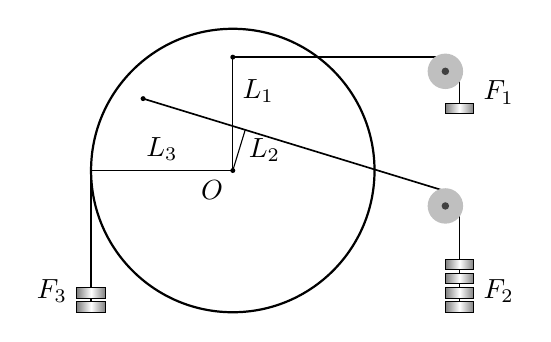
\begin{tikzpicture}[>=latex,scale=0.9]
  % \useasboundingbox(-1.2,-3.55)rectangle(1.2,3.15);
  \tkzDefPoints{0/0/O,0/0.4/A,3.0/-0.5/O2,3.0/1.4/O1}
  \tkzDefTangent[from=O2](O,A)\tkzGetPoints{B'}{B}
  \tkzDefPointBy[translation=from O to B](O2)\tkzGetPoint{M}
  \tkzDefMidPoint(O2,M)\tkzGetPoint{T}
  \tkzDefPointBy[projection = onto O--B](T)\tkzGetPoint{T'}
  \tkzDefPointOnLine[pos=1.5](T,T')\tkzGetPoint{P}
  \draw[semithick](T)--(P);
  \draw[thick](O)circle(2);
  \draw[semithick](0,1.6)--(3,1.6)(3.2,1.4)--(3.2,0.8)(-2,0)--(-2,-2)(3.2,-0.5)--(3.2,-2);
  \foreach \x in {-2,-1.8}
  {
    \fill[left color=gray,right color=gray,middle color=white,draw=black,thin]
    (-2.2,\x)rectangle(-1.8,\x+0.15);
    \fill[left color=gray,right color=gray,middle color=white,draw=black,thin]
    (3.0,\x)rectangle(3.4,\x+0.15);
    \fill[left color=gray,right color=gray,middle color=white,draw=black,thin]
    (3.0,\x+0.4)rectangle(3.4,\x+0.55);
  }
  \fill[left color=gray,right color=gray,middle color=white,draw=black,thin]
    (3.0,0.8)rectangle(3.4,0.95);
  \draw[thin](0,0)--(-2,0)node[midway,above]{$L_3$};
  \draw[thin](0,0)--(0,1.6)node[pos=0.7,right]{$L_1$};
  \draw[thin](O)--(T')node[midway,,right]{$L_2$};
  \fill(0,0)circle(1pt)node[below left]{$O$};
  \fill(0,1.6)circle(1pt);
  \fill(P)circle(1pt);
  \fill[lightgray](O1)circle(0.25);
  \fill[lightgray](O2)circle(0.25);
  \fill[darkgray](O1)circle(1.5pt);
  \fill[darkgray](O2)circle(1.5pt);
  \node at (-2.2,-2)[above left]{$F_3$};
  \node at (3.4,-2)[above right]{$F_2$};
  \node at (3.4,0.8)[above right]{$F_1$};
\end{tikzpicture}
\end{document}